\section{Evaluation}
\subsection{YOLO Object Detection}
Our main goal is to never miss the detection of a potential license plate. This
means that we favor recall over precision, which means that we want the correct
license plate amongst the set of detected objects even if this means an
increased number of false positives.

Our solution achieves \todo{}$\%$ precision on our test data. test

\begin{figure}
    \begin{subfigure}[b]{.55\textwidth}
        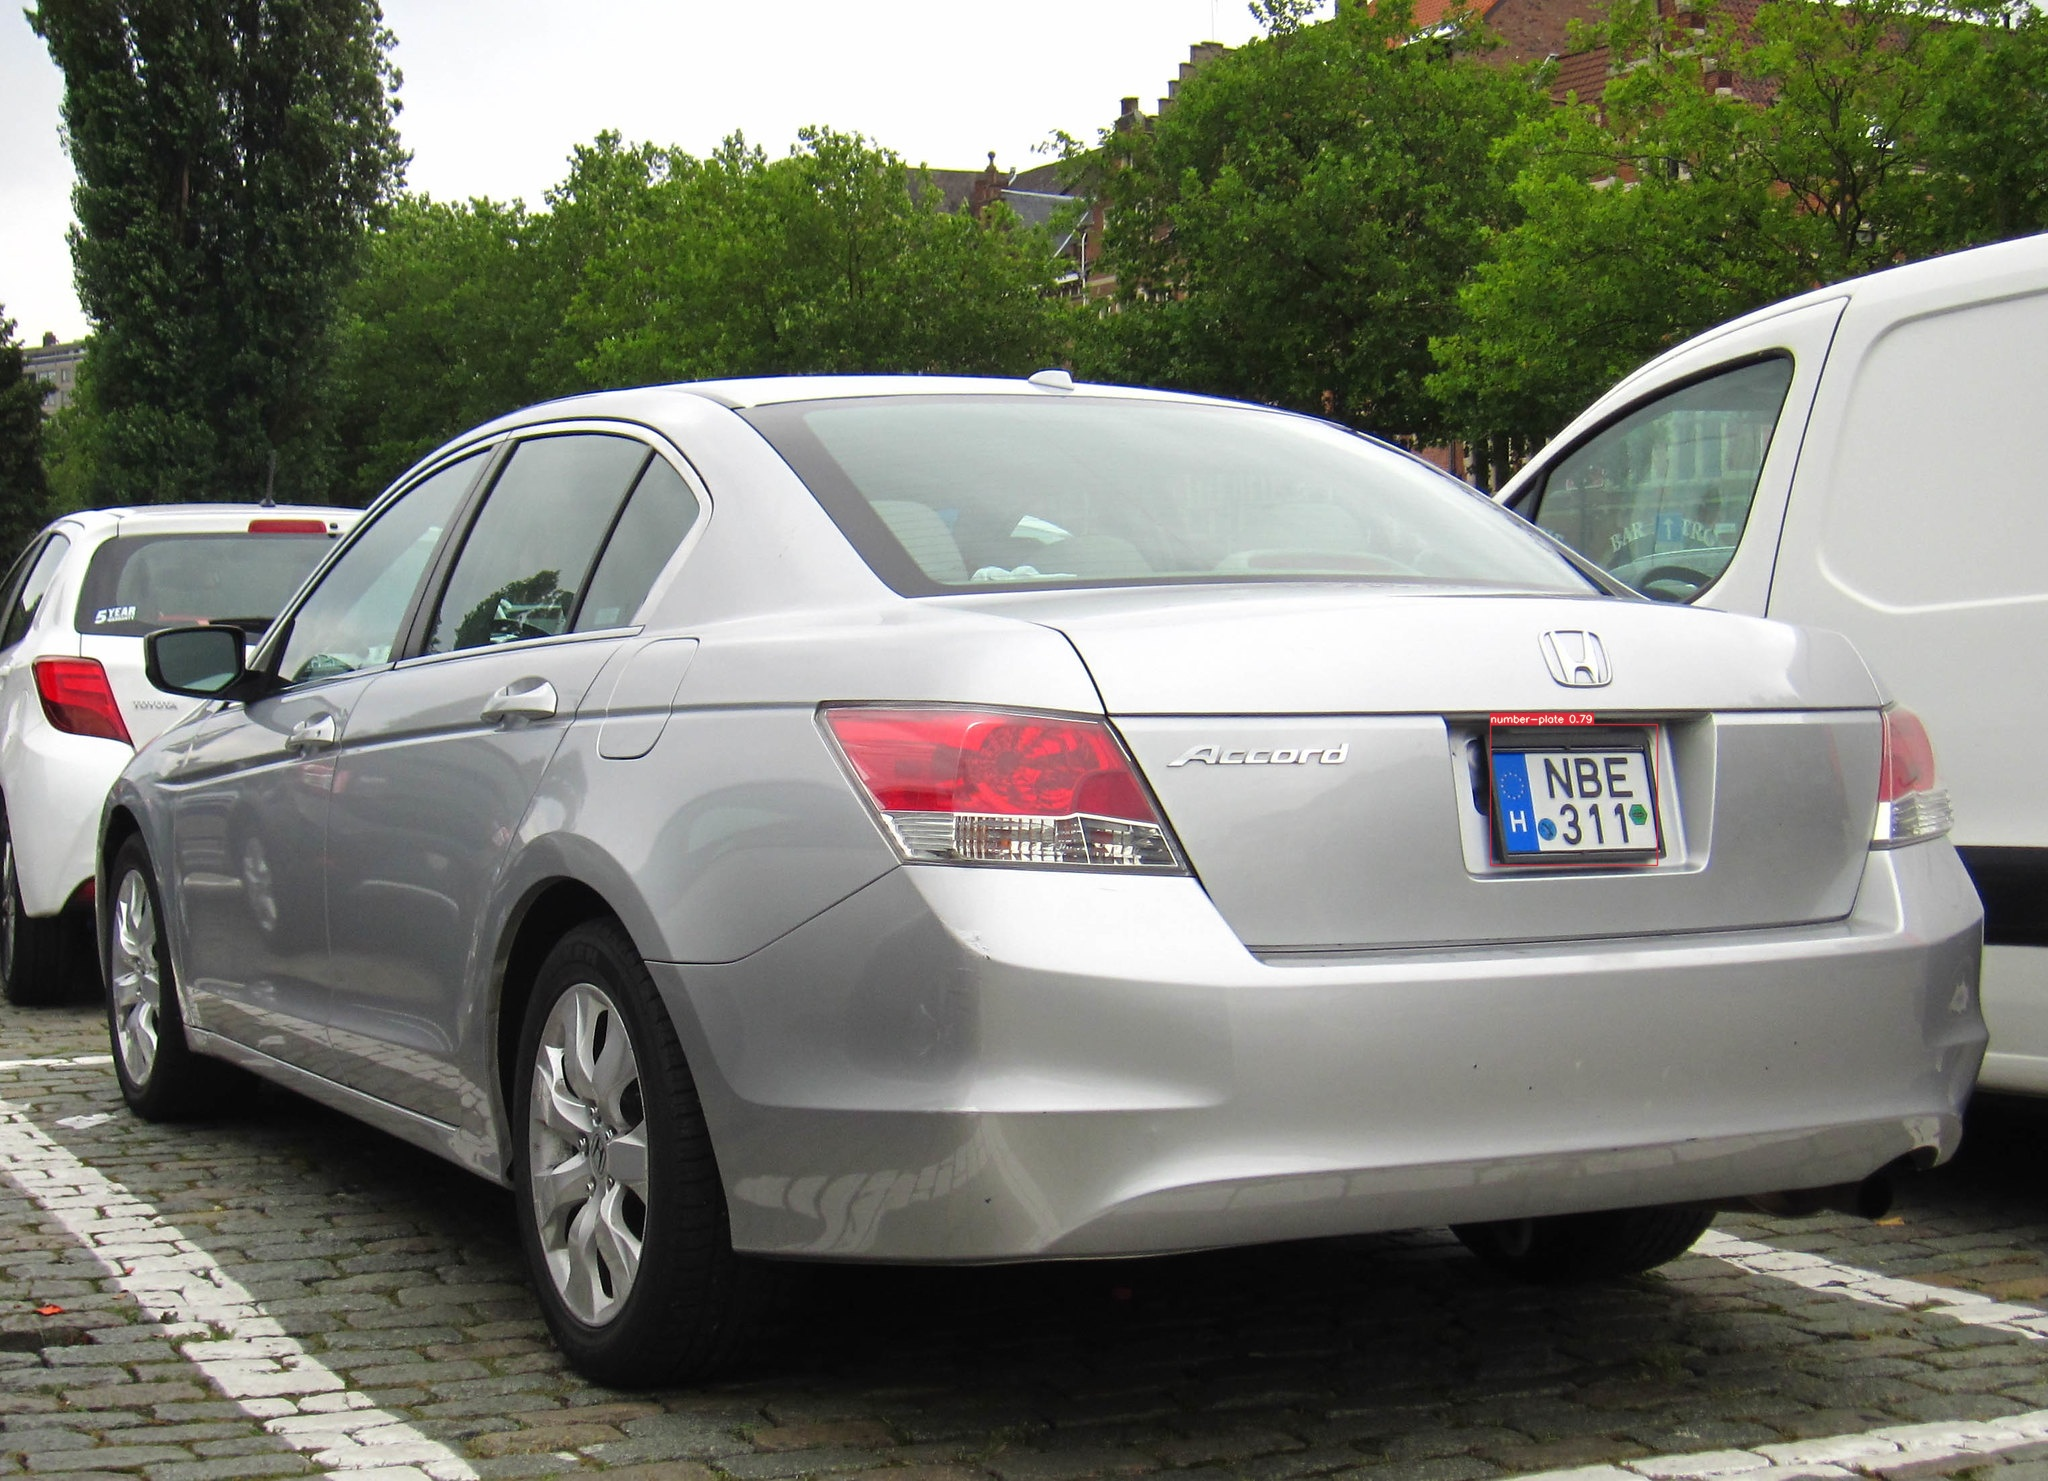
\includegraphics[width=\textwidth]{figures/yolo/1000.jpg}
    \end{subfigure}
    \hfill
    \begin{subfigure}[b]{.15\textwidth}
        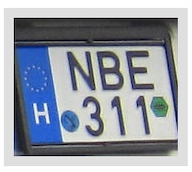
\includegraphics[width=\textwidth]{figures/yolo/1000_montage.png}
    \end{subfigure}
    \hfill\hfill
    \\
    \begin{subfigure}[b]{.55\textwidth}
        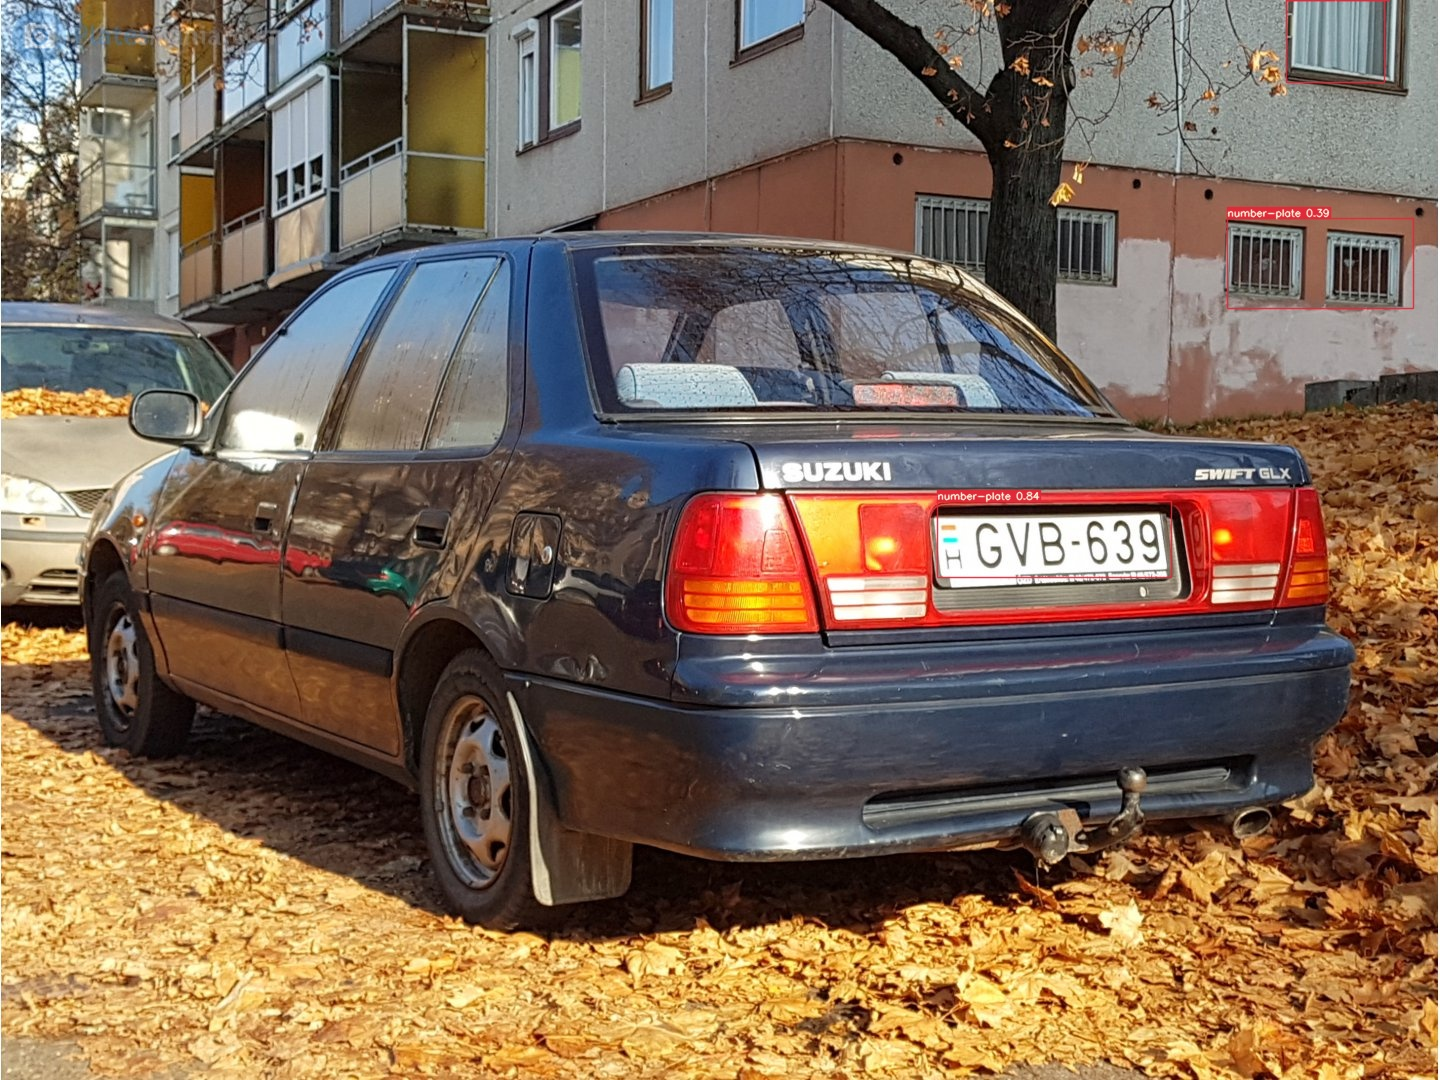
\includegraphics[width=\textwidth]{figures/yolo/179.jpg}
    \end{subfigure}
    \hfill
    \begin{subfigure}[b]{.4\textwidth}
        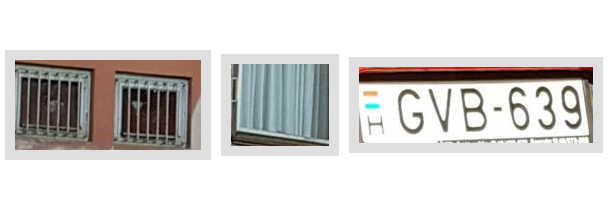
\includegraphics[width=\textwidth]{figures/yolo/179_montage.png}
    \end{subfigure}
    \hfill
    \caption{Example YOLO detections, and the corresponding cut outs.
        Background elements might get incorrectly labeled as number plates.  As
        we mention later on, our goal is to get a high as possible recall. If
        a lower false positive count was desired, we could increase the
    confidence threshold.}
    \label{fig:yolo-detection-montages}
\end{figure}

Figure~\ref{fig:yolo-detection-montages}  shows random detections in different
scenarios. We cut out each of the detected objects to separate image files. Some
examples can be seen on Figure~\ref{fig:cutout-montage}.
These cut out detections serve as the input of the next step of our \ac{ALPR}
pipeline.
\begin{figure}
    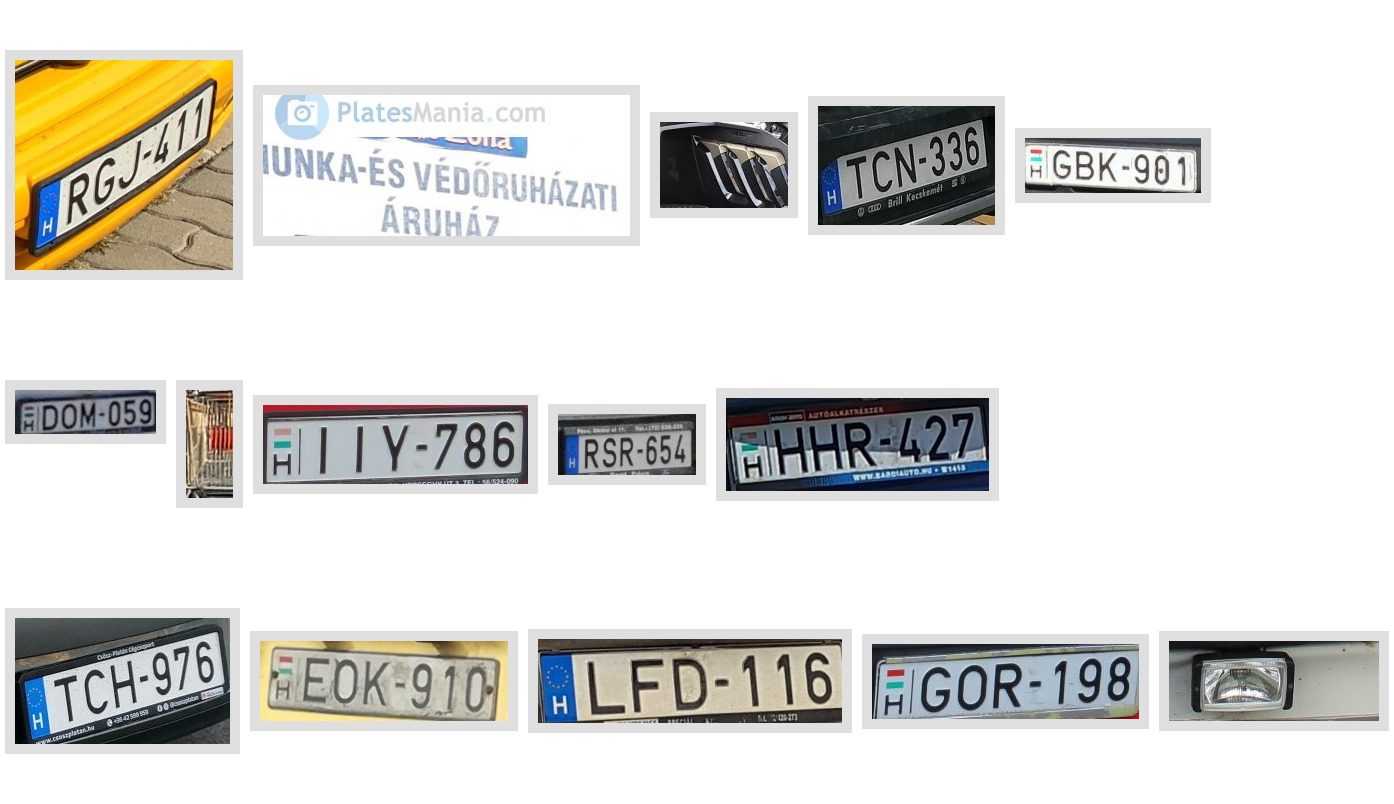
\includegraphics[width=\textwidth]{figures/yolo/cutout_montage.jpg}
    \caption{Some example object detection results that serve as the
    input for the OCR stage.}
    \label{fig:cutout-montage}
\end{figure}

\subsection{Optical Character Recognition (OCR)}

When it comes to \ac{OCR} we first tried to train our own \ac{NN}.  We have
based our work on the architecture described in Shi et al. \cite{7801919}.
Unfortunately in the end this endeavour did not succeed.  We have gained a lot
of insight into the given pipeline.  Some parts of this \ac{OCR} implementation
worked successfully.  First we trained this \ac{NN} with automatically generated
text samples.  The text generation was achieved with a \emph{Python} console
application called \emph{trdg}.  This allowed us to generate images based on
a text document.  These images contained noise and different levels of
distortions.  This was meant to precede the training on real world data.

We also experimented with different data augmentation methods.  These methods
included changing the lighting conditions, skewing images, applying noise and
others.  One of the used augmentation algorithms is capable of changing the
weather conditions of the scene on the picture.  Besides applying distortions
for data augmentation purposes, we have used inverse, denoising methods to
improve the confidence of the recognition process.

After successful training and testing on the automatically generated data, we
decided to train our model on the real world images.  We used the provided test
database containing cars with Hungarian license plates.  The \ac{NN} was trained
for hundred epochs.  Each epoch contained fifty batches of images.  One batch
contained thirty-five images.  After this amount of training the model began to
struggle to further decrease the loss.  At this point we decided to use
a different model.  In the final application we use the \emph{PaddleOCR}
\cite{DBLP:journals/corr/abs-2009-09941}.

\subsection{Qualitative Comparison}
For qualitative comparison, we consider scenarios with viewing conditions
corresponding to more difficult visual settings. We categorize these cases by
perceived difficulty, and show examples. Figure \todo{add figure} shows
different settings. \todo[inline]{Evaluate which one is the hardest setting.}

These are some of the settings we expect to make \ac{ALPR} more
difficult:
\begin{itemize}
    \item Direct sunlight 
    \item Partial occlusion of the license plate 
    \item Miscellaneous weather effects such as rain or fog
    \item Small size of the licence plate (i.e. the object is further away)
\end{itemize}

We implemented these effects in OpenCV. 
\todo[inline]{refernce weather comparison}
